\section{Existing applications}

We managed to find some applications, but also platforms allowing you to build your own application.

	\subsection{Bluebridge}
	Bluebridge is a provider of tourism applications. It provides :
	\begin{itemize}
		\item  Back-end technology (platform) to power your app
		\item  Mobile App Studio CMS (product) to design your app
		\item  Best-in-class app packages
		\item  Professional services
		\item  A message center to manage push notifications
	\end{itemize}

The platform is a Software as a service, using its own technology, so we don't have any way to know how they are implemented. But the features proposed on the website are interesting, so we will developp them.

\paragraph{GPS locating} As far as we thought, the GPS location is one of the main features when you want to implement an applications creating tours. Of course we can decide not to use it, and just display the best way between the monuments the user chose. This would mean that we assume that the user can find the first monument of the tour alone, and then will manage to find easily the way the application displays.
\begin{figure}[h!]
	\centering
	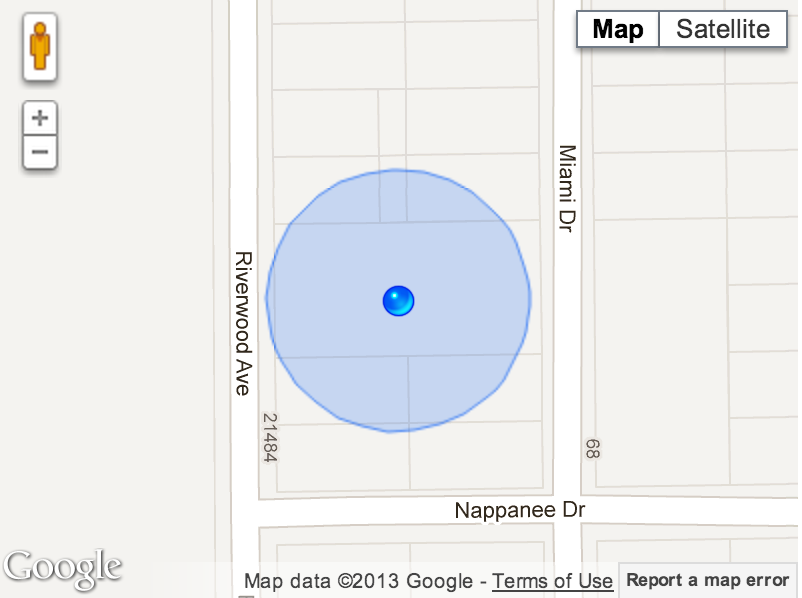
\includegraphics[scale=0.37]{input/current-location.png}
	\caption{Google Maps displaying your location.}
	\label{fig:location}
\end{figure}
The GPS location will allow the user to know where he is and to confirm he goes in the right direction.


\paragraph{GPS directions} This function is complementary with displaying the way between two monuments. Thanks to the GPS directions, the user can just be guided by the GPS, telling him which street he is currently in, where and when he should turn. Of course it will also announce his arrival to the monument he selected. It's not a compulsory feature, but it sure is a convenient one.
\begin{figure}[h!]
	\centering
	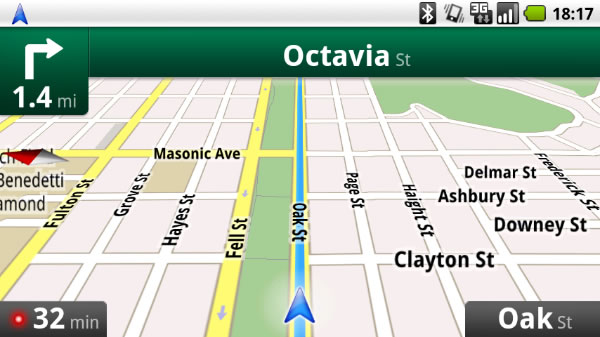
\includegraphics[width=0.6\textwidth]{input/directions.png}
	\caption{Google Maps displaying the navigation directions.}
	\label{fig:directions}
\end{figure}
Since Bluebridge is not a real application, those are the main features we found. They are pretty classic so we won't present them in other applications. Let's head to the second application.

\paragraph{Itinerary planner} It seems like the main idea of our application already exists. This feature is called Itinerary planner in Bluebridge, and give the users the option to set an attraction as `` favorite ''. When added as so, the attraction is added to a tab where users can plan their stay. It also gives the quicker route to the favorite attractions.


\paragraph{Experience guides} This is a real little guide within the application. It can contain several things, such as :
\begin{itemize}
	\item One-touch, turn-by-turn directions to attractions (interactive tours)
  \item Featured photos
  \item Content about local happenings
  \item Exclusive discounts and offers
\end{itemize}

In our application, only one seems to be interesting. We don't want our application to be a guide for visiting the place you are in, we just want the best way to join the places the user selected. But it can be nice, and also help  the user to recognize the place, to display some pictures of the place the user is heading to. It would be a kind of preview that could better a little the design of the application, and for this reason it is worth thinking about implementing it.


Here were the most important and interesting features of the provider Bluebridge. We will now discover another provider which offer other types of features.

\newpage{}\subsection{mTrip}
mTrip is a company specialized in the development of tourism applications. Their applications have been downloaded over 2.5 million times, thanks to some special features like :
\begin{itemize}
	\item Offline content
	\item Augmented reality
  \item Nearby places
  \item Currency converter
  \item Trip journal
  \item Sharing features
\end{itemize}

We won't be interested in all of them, only 3 of them will be developed in the following paragraphs.

\paragraph{Offline content} We can note the offline content, that is really interesting because it allows the user to access data on the application without being connected to the Internet. Our application, and more generally tourism applications are meant to be used abroad, where roaming fees are high and you don't want to be connected too often. But the data has to be stored within the application, which can make it a big application to download.


\paragraph{Augmented reality} Augmented reality will not be useful in our case, but the aim of this feature is to allow the user to visualize the place he wants to visit, or the way to go to it. Since we assume the plan we provide, with name of the streets, the distance to go and GPS directions, we assume it is enough to have a clear idea of where you should go. A preview of the monuments can be done with the pictures we saw above.


\paragraph{Nearby places} Displaying the nearby places is also a classical feature, it can be interesting to implement it. For example, during the tour you organized, the user can realize that he is close to another building that he thought he won't have the time to visit, or maybe just he didn't thought about. It adds many possibility of unscheduled visits to the user, and will really improve the quality of the service offered by our application.

With those two application providers, we have a pretty complete overview of what tourism applications can contain, the essential features they should contain and what is useful to implement or not. We will now present our analyze of the Google Maps API.




